% Created 2024-02-12 Mon 09:15
% Intended LaTeX compiler: pdflatex
\documentclass[presentation, aspectratio=1610]{beamer}
\usepackage[utf8]{inputenc}
\usepackage[T1]{fontenc}
\usepackage{graphicx}
\usepackage{longtable}
\usepackage{wrapfig}
\usepackage{rotating}
\usepackage[normalem]{ulem}
\usepackage{amsmath}
\usepackage{amssymb}
\usepackage{capt-of}
\usepackage{hyperref}
\usetheme[progressbar=foot]{metropolis}
\usepackage[sorting=ynt]{biblatex}
\addbibresource{../src/myBib.bib}
\usepackage{caption}
\captionsetup[figure]{labelformat=empty}
\DeclareMathOperator*{\argmax}{\arg\!max}
\DeclareMathOperator*{\argmin}{\arg\!min}
\AtBeginSubsection{\begin{frame}\tableofcontents[currentsection,currentsubsection]\end{frame}}
\usetheme{metropolis}
\usecolortheme{}
\usefonttheme{}
\useinnertheme{}
\useoutertheme{}
\author{Andrew Jensen}
\date{March 9, 2023}
\title{Joint Track Machine Learning}
\hypersetup{
 pdfauthor={Andrew Jensen},
 pdftitle={Joint Track Machine Learning},
 pdfkeywords={},
 pdfsubject={},
 pdfcreator={Emacs 29.1 (Org mode 9.7)}, 
 pdflang={English}}
\begin{document}

\maketitle
\begin{frame}{Outline}
\tableofcontents
\end{frame}

\begin{frame}[label={sec:org9eecd50},standout]{Acknowledgments}
I would like to thank the McJunkin Family Charitable Foundation for their generous grant that supports this work.
\end{frame}
\begin{frame}[label={sec:org2b7cb7e}]{The Problem}
\begin{columns}
\begin{column}{0.5\columnwidth}
\begin{itemize}
\item By 2030, roughly 3.5 million Total Knee Arthroplasty (TKA) will be performed in the US \autocite{kurtzProjectionsPrimaryRevision2007}.
\item 20\% of patients receiving TKA are dissatisfied.
\begin{itemize}
\item Instability, pain, unnatural \autocites{bakerRolePainFunction2007}[][]{bournePatientSatisfactionTotal2010}[][]{scottPredictingDissatisfactionFollowing2010}.
\end{itemize}
\item No reliable method of clinically assessing and quantifying joint dynamics.
\begin{itemize}
\item Human supervision
\item Time consuming
\item Specialized equipment
\end{itemize}
\end{itemize}
\end{column}
\begin{column}{0.5\columnwidth}
\begin{center}
\includegraphics[width=\textwidth]{/home/ajensen123@ad.ufl.edu/repo/lit-review/figures/raster/Physical_Examination_of_the_knee.jpg}
\end{center}
\end{column}
\end{columns}
\end{frame}
\begin{frame}[label={sec:orgc484a76}]{Our Proposition}
\begin{columns}
\begin{column}{0.5\columnwidth}
Orthopaedic surgeons and clinicians would readily adopt a \alert{\alert{practical}} and \alert{\alert{inexpensive}} technology that allows them to \alert{\alert{measure}} a patient's knee kinematics during \alert{\alert{activities of daily living}}.
\end{column}
\begin{column}{0.55\columnwidth}
\begin{center}
\includegraphics[width=2in]{/home/ajensen123@ad.ufl.edu/repo/lit-review/figures/raster/dynamic-knee-prescription.png}
\end{center}
\end{column}
\end{columns}
\end{frame}
\begin{frame}[label={sec:orgdba89f4}]{Constraints}
\begin{columns}
\begin{column}{0.45\columnwidth}
\begin{itemize}
\item It must fit within a \alert{\alert{standard clinical workflow}}
\item The technology must utilize equipment \alert{\alert{commonly found in hospitals}}
\item There must not be significant \alert{\alert{human supervision}} nor interaction to generate an examination report.
\end{itemize}
\end{column}
\begin{column}{0.55\columnwidth}
\begin{center}
\includegraphics[width=\textwidth]{/home/ajensen123@ad.ufl.edu/repo/lit-review/figures/raster/c-arm-fluoro-machine.jpg}
\end{center}
\end{column}
\end{columns}
\end{frame}
\begin{frame}[label={sec:org3380b5c}]{Background - Projective Geometry}
\begin{center}
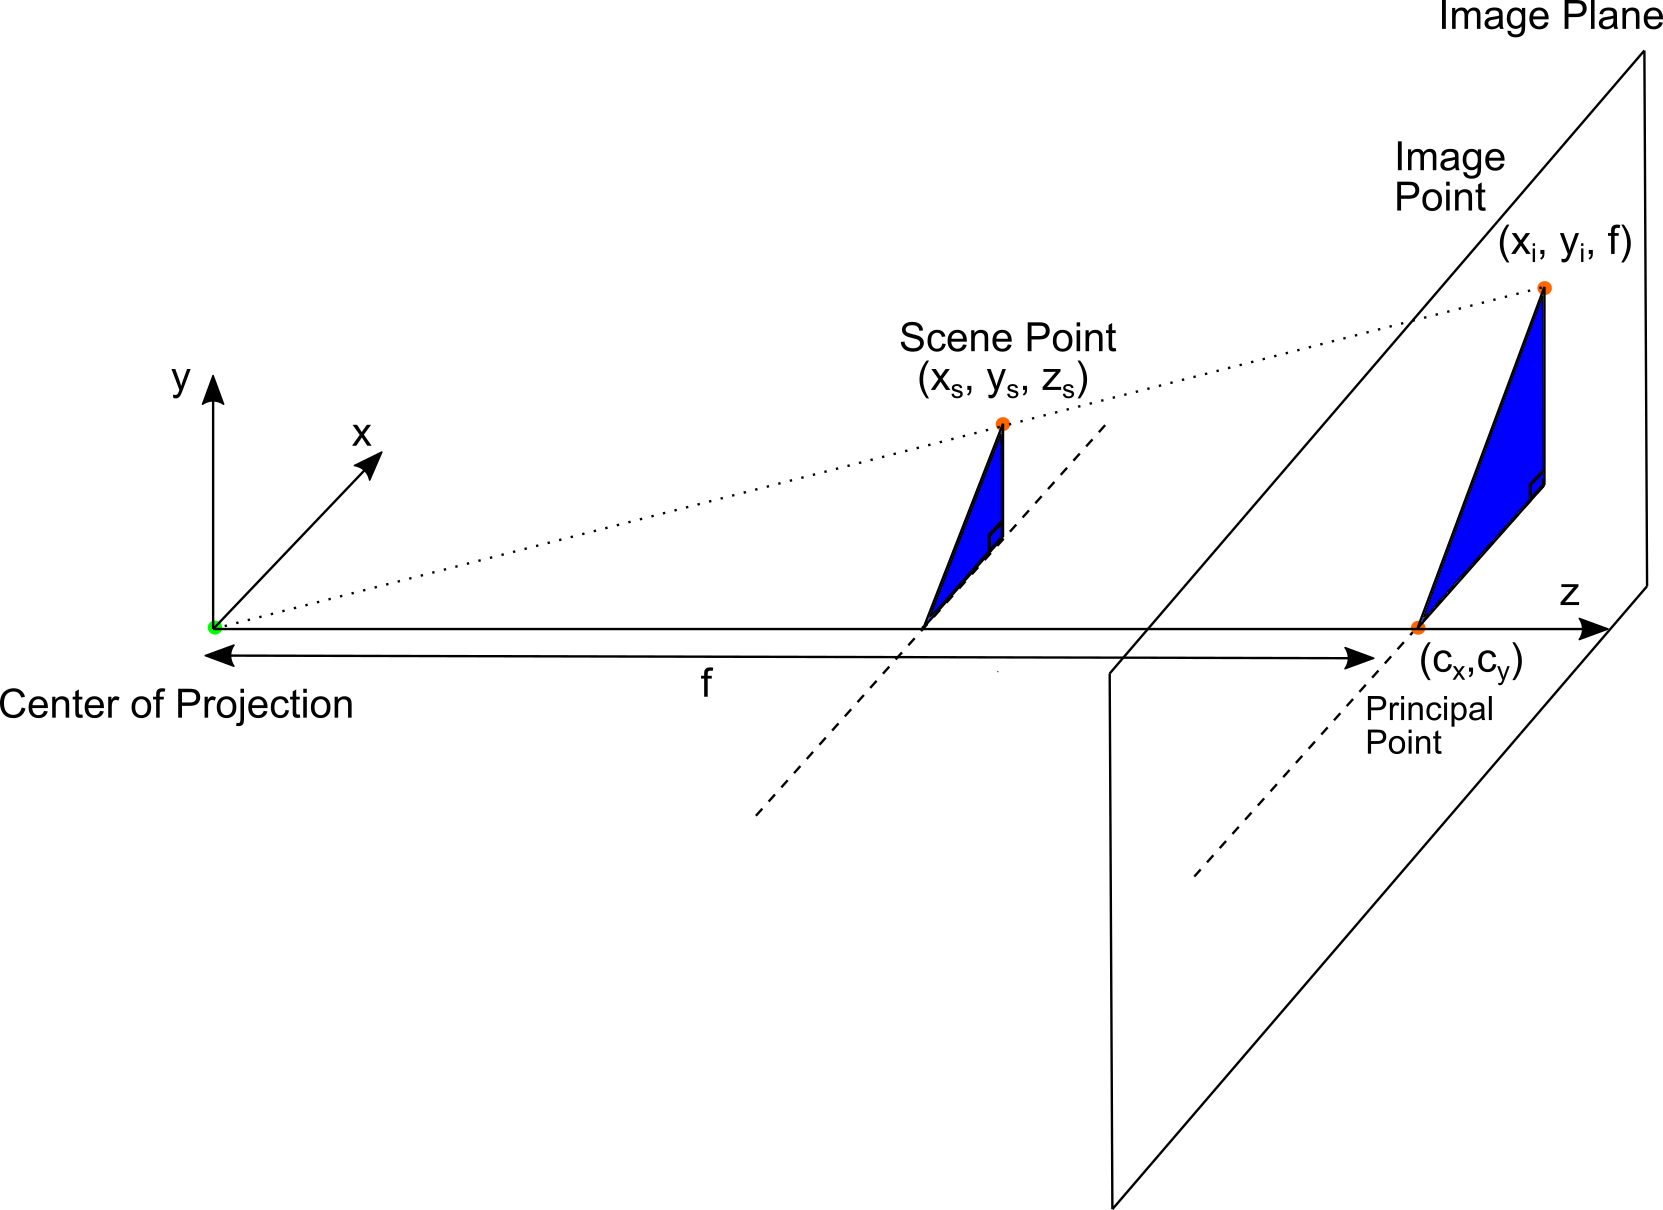
\includegraphics[width=0.8\textwidth]{/home/ajensen123@ad.ufl.edu/repo/lit-review/figures/raster/perspective-projection.png}
\end{center}
\end{frame}
\begin{frame}[label={sec:org2154104}]{Background - Model-Image Registration}
\begin{columns}
\begin{column}{0.5\columnwidth}
If we know the projective parameters of the fluoroscopy machine, can we tinker with \(T^{cam}_{implant}\) so that our virtual projection matches the fluoroscopic image?
\end{column}
\begin{column}{0.6\columnwidth}
\begin{figure}[htbp]
\centering
\includegraphics[width=2.5in]{/home/ajensen123@ad.ufl.edu/repo/lit-review/figures/raster/registered-tka.png}
\caption{From \autocite{mahfouzRobustMethodRegistration2003}}
\end{figure}
\end{column}
\end{columns}
\end{frame}
\begin{frame}[label={sec:org1998fec}]{Background - Model-Image Registration}
\begin{columns}
\begin{column}{0.5\columnwidth}
If we know the projective parameters of the fluoroscopy machine, can we tinker with \(T^{cam}_{implant}\) so that our virtual projection matches the fluoroscopic image?
\end{column}
\begin{column}{0.6\columnwidth}
\begin{figure}[htbp]
\centering
\includegraphics[width=2.5in]{/home/ajensen123@ad.ufl.edu/repo/lit-review/figures/raster/mahfouz-perspective-projection.png}
\caption{From \autocite{mahfouzRobustMethodRegistration2003}}
\end{figure}
\end{column}
\end{columns}
\end{frame}
\begin{frame}[label={sec:org221d9f4}]{Historical Overview}
Many different approaches have attempted to solve the model-image registration problem.
\begin{itemize}
\item Pre-computed projections
\item Skin-mounted motion Capture
\item Biplane Imaging
\item Iterative Projections
\item Roentgen Stereophotogrammetry
\end{itemize}
\end{frame}
\begin{frame}[label={sec:org93f2248}]{Pre-Computed Projections}
\begin{columns}
\begin{column}{0.5\columnwidth}
\begin{itemize}
\item Saving space and memory by pre-computing as much as possible.
\item Pre-computed distance maps \autocites{zuffiModelbasedMethodReconstruction1999}[][]{lavalleeRecoveringPositionOrientation1995}.
\item Pre-computed shape libraries \autocite{banksAccurateMeasurementThreedimensional1996}
\end{itemize}
\end{column}
\begin{column}{0.6\columnwidth}
\begin{figure}[htbp]
\centering
\includegraphics[width=1.75in]{/home/ajensen123@ad.ufl.edu/repo/lit-review/figures/raster/lavallee-distance-maps.png}
\caption{From \autocite{lavalleeRecoveringPositionOrientation1995}}
\end{figure}
\begin{figure}[htbp]
\centering
\includegraphics[width=1.75in]{/home/ajensen123@ad.ufl.edu/repo/lit-review/figures/raster/banks-nfd-library.png}
\caption{From \autocite{banksAccurateMeasurementThreedimensional1996}}
\end{figure}
\end{column}
\end{columns}
\end{frame}
\begin{frame}[label={sec:orgbba6e05}]{Limitations of Pre-Computed Projections}
\begin{columns}
\begin{column}{0.5\columnwidth}
\begin{itemize}
\item Requires an accurate contour from the input image in order to perform calculations.
\begin{itemize}
\item Human supervision for isolated contour
\item Inaccuaracy with naive edge detection
\end{itemize}
\end{itemize}
\end{column}
\begin{column}{0.6\columnwidth}
\begin{figure}[htbp]
\centering
\includegraphics[width=1.75in]{/home/ajensen123@ad.ufl.edu/repo/lit-review/figures/raster/lavallee-distance-maps.png}
\caption{From \autocite{lavalleeRecoveringPositionOrientation1995}}
\end{figure}
\begin{figure}[htbp]
\centering
\includegraphics[width=1.75in]{/home/ajensen123@ad.ufl.edu/repo/lit-review/figures/raster/banks-nfd-library.png}
\caption{From \autocite{banksAccurateMeasurementThreedimensional1996}}
\end{figure}
\end{column}
\end{columns}
\end{frame}
\begin{frame}[label={sec:org697ebb4}]{Motion Capture (MoCap)}
\begin{columns}
\begin{column}{0.5\columnwidth}
\begin{itemize}
\item Can measure motion of MoCap beads very accurately.
\item Skin-mounted \autocites{gaoInvestigationSoftTissue2008}[][]{kuoInfluenceSoftTissue2011}[][]{linEffectsSoftTissue2016}.
\item Bone pins \autocite{lafortuneThreedimensionalKinematicsHuman1992}.
\end{itemize}
\end{column}
\begin{column}{0.6\columnwidth}
\begin{figure}[htbp]
\centering
\includegraphics[width=2.5in]{/home/ajensen123@ad.ufl.edu/repo/lit-review/figures/raster/gao-skin-mocap.png}
\caption{From \autocite{gaoInvestigationSoftTissue2008}}
\end{figure}
\begin{figure}[htbp]
\centering
\includegraphics[width=2.5in]{/home/ajensen123@ad.ufl.edu/repo/lit-review/figures/raster/lafortune-bone-mocap.png}
\caption{From \autocite{lafortuneThreedimensionalKinematicsHuman1992}}
\end{figure}
\end{column}
\end{columns}
\end{frame}
\begin{frame}[label={sec:orgb12eb38}]{Limitations of Motion Capture}
\begin{columns}
\begin{column}{0.5\columnwidth}
Skin Mounted
\begin{itemize}
\item Doesn't accurately describe underlying skeletal motion with clinical accuracy \autocites{gaoInvestigationSoftTissue2008}[][]{kuoInfluenceSoftTissue2011}[][]{linEffectsSoftTissue2016}.
\end{itemize}
Bone Pins
\begin{itemize}
\item Any volunteers?
\end{itemize}
\end{column}
\begin{column}{0.6\columnwidth}
\begin{figure}[htbp]
\centering
\includegraphics[width=2.5in]{/home/ajensen123@ad.ufl.edu/repo/lit-review/figures/raster/gao-skin-mocap.png}
\caption{From \autocite{gaoInvestigationSoftTissue2008}}
\end{figure}
\begin{figure}[htbp]
\centering
\includegraphics[width=2.5in]{/home/ajensen123@ad.ufl.edu/repo/lit-review/figures/raster/lafortune-bone-mocap.png}
\caption{From \autocite{lafortuneThreedimensionalKinematicsHuman1992}}
\end{figure}
\end{column}
\end{columns}
\end{frame}
\begin{frame}[label={sec:orgd10cc65}]{Biplane Imaging}
\begin{columns}
\begin{column}{0.5\columnwidth}
\begin{itemize}
\item Utilizes multiple cameras to resolve 3D position and orientation\autocites{ivesterReconfigurableHighSpeedStereoRadiography2015}[][]{burtonAutomaticTrackingHealthy2021}.
\begin{itemize}
\item Highly accurate.
\item Gold Standard.
\end{itemize}
\end{itemize}
\end{column}
\begin{column}{0.6\columnwidth}
\begin{figure}[htbp]
\centering
\includegraphics[width=1.75in]{/home/ajensen123@ad.ufl.edu/repo/lit-review/figures/raster/ivester-stereo-fluoromachine.png}
\caption{Both from \autocite{ivesterReconfigurableHighSpeedStereoRadiography2015}}
\end{figure}
\begin{figure}[htbp]
\centering
\includegraphics[width=1.75in]{/home/ajensen123@ad.ufl.edu/repo/lit-review/figures/raster/ivester-stereo-projection.png}
\end{figure}
\end{column}
\end{columns}
\end{frame}
\begin{frame}[label={sec:org200e647}]{Limitations of Biplane Imaging}
\begin{columns}
\begin{column}{0.5\columnwidth}
\begin{itemize}
\item Not many hospitals have biplane fluoroscopy setups.
\item Clinically impractical
\end{itemize}
\end{column}
\begin{column}{0.6\columnwidth}
\begin{figure}[htbp]
\centering
\includegraphics[width=1.75in]{/home/ajensen123@ad.ufl.edu/repo/lit-review/figures/raster/ivester-stereo-fluoromachine.png}
\caption{Both from \autocite{ivesterReconfigurableHighSpeedStereoRadiography2015}}
\end{figure}
\begin{figure}[htbp]
\centering
\includegraphics[width=1.75in]{/home/ajensen123@ad.ufl.edu/repo/lit-review/figures/raster/ivester-stereo-projection.png}
\end{figure}
\end{column}
\end{columns}
\end{frame}
\begin{frame}[label={sec:org1732476}]{Iterative Projections}
\begin{columns}
\begin{column}{0.54\columnwidth}
\begin{itemize}
\item Take advantage of modern computational graphics pipelines to quickly perform projection matching.
\begin{itemize}
\item Image/Intensity similarity metrics \autocite{mahfouzRobustMethodRegistration2003}
\item Feature/Contour similarity metrics \autocite{floodAutomatedRegistration3D2018}
\end{itemize}
\end{itemize}
\end{column}
\begin{column}{0.6\columnwidth}
\begin{figure}[htbp]
\centering
\includegraphics[width=2in]{/home/ajensen123@ad.ufl.edu/repo/lit-review/figures/raster/mahfouz-perspective-projection.png}
\caption{From \autocite{mahfouzRobustMethodRegistration2003}}
\end{figure}
\begin{figure}[htbp]
\centering
\includegraphics[width=2in]{/home/ajensen123@ad.ufl.edu/repo/lit-review/figures/raster/flood-dilated-contour.png}
\caption{From \autocite{floodAutomatedRegistration3D2018}}
\end{figure}
\end{column}
\end{columns}
\end{frame}
\begin{frame}[label={sec:org5d0b2c9}]{Limitations of (historic) Iterative Projection Methods}
\begin{columns}
\begin{column}{0.54\columnwidth}
\begin{itemize}
\item Requires human supervision for:
\begin{itemize}
\item Pose initialization
\item Escaping local minima
\item Implant detection
\end{itemize}
\item Chaotic and Noisy objective function
\end{itemize}
\end{column}
\begin{column}{0.6\columnwidth}
\begin{figure}[htbp]
\centering
\includegraphics[width=2in]{/home/ajensen123@ad.ufl.edu/repo/lit-review/figures/raster/mahfouz-perspective-projection.png}
\caption{From \autocite{mahfouzRobustMethodRegistration2003}}
\end{figure}
\begin{figure}[htbp]
\centering
\includegraphics[width=2in]{/home/ajensen123@ad.ufl.edu/repo/lit-review/figures/raster/flood-dilated-contour.png}
\caption{From \autocite{floodAutomatedRegistration3D2018}}
\end{figure}
\end{column}
\end{columns}
\end{frame}
\begin{frame}[label={sec:org51e908f}]{Roentgen Stereophotogrammetry (RSA)}
\begin{columns}
\begin{column}{0.5\columnwidth}
\begin{itemize}
\item Uses implanted tantalum beads for motion tracking \autocites{vroomanFastAccurateAutomated1998}[][]{selvikRoentgenStereophotogrammetryMethod1989}
\item Extremely accurate \autocites{kapteinEvaluationThreePose2004}[][]{saariKneeKinematicsMedial2005}
\item Gold standard Measurement \autocite{brobergValidationMachineLearning2023}
\end{itemize}
\end{column}
\begin{column}{0.6\columnwidth}
\begin{figure}[htbp]
\centering
\includegraphics[width=3in]{/home/ajensen123@ad.ufl.edu/repo/lit-review/figures/raster/vrooman-mbrsa.png}
\caption{From \autocite{vroomanFastAccurateAutomated1998}}
\end{figure}
\end{column}
\end{columns}
\end{frame}
\begin{frame}[label={sec:org0b7fc7a}]{Limitations of RSA}
\begin{columns}
\begin{column}{0.5\columnwidth}
\begin{itemize}
\item Involves additional surgical procedures for inserting tantalum beads.
\item Human supervision
\item Bi-plane imaging
\end{itemize}
\end{column}
\begin{column}{0.6\columnwidth}
\begin{figure}[htbp]
\centering
\includegraphics[width=3in]{/home/ajensen123@ad.ufl.edu/repo/lit-review/figures/raster/vrooman-mbrsa.png}
\caption{From \autocite{vroomanFastAccurateAutomated1998}}
\end{figure}
\end{column}
\end{columns}
\end{frame}
\section{Aims}
\label{sec:org36b0efc}
\begin{frame}[label={sec:orgc351f3e}]{Aims}
\begin{columns}
\begin{column}{0.3\columnwidth}
\begin{block}{Aims 1/2}
Joint Track Machine Learning and Overcoming Single-Plane Limitations
\end{block}
\end{column}
\begin{column}{0.3\columnwidth}
\begin{block}{Aim 3/4}
Pilot Trials and Standardized Kinematics Exam
\end{block}
\end{column}
\begin{column}{0.3\columnwidth}
\begin{block}{Aim 5}
Joint Track Auto Toolkit
\end{block}
\end{column}
\end{columns}
\end{frame}
\subsection{Aim 1 - Joint Track Machine Learning}
\label{sec:org397b883}
\begin{frame}[label={sec:org04a3a88}]{Goal}
Demonstrate the feasibility of a fully autonomous, model-image registration pipeline.
\end{frame}
\begin{frame}[label={sec:orgfa9da2d}]{Method}
\begin{itemize}
\item Three-tiered approach
\begin{itemize}
\item Convolutional Neural networks (CNN) for autonomous implant detection
\item Normalized Fourier Descriptor shape libraries
\item Robust contour-based global optimization scheme
\end{itemize}
\end{itemize}
\begin{center}
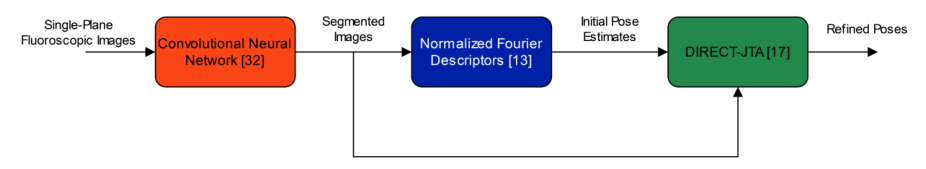
\includegraphics[width=\textwidth]{/home/ajensen123@ad.ufl.edu/repo/lit-review/figures/raster/jtml-pipeline.png}
\end{center}
\end{frame}
\begin{frame}[label={sec:orgc8769ae}]{Autonomous Implant Detection Using Convolutional Neural Networks}
\begin{columns}
\begin{column}{0.5\columnwidth}
\begin{itemize}
\item 2 CNNs
\begin{itemize}
\item Femoral and Tibial implants
\end{itemize}
\item High Resolution Network \autocite{wangDeepHighResolutionRepresentation2020}
\end{itemize}
\end{column}
\begin{column}{0.5\columnwidth}
\begin{center}
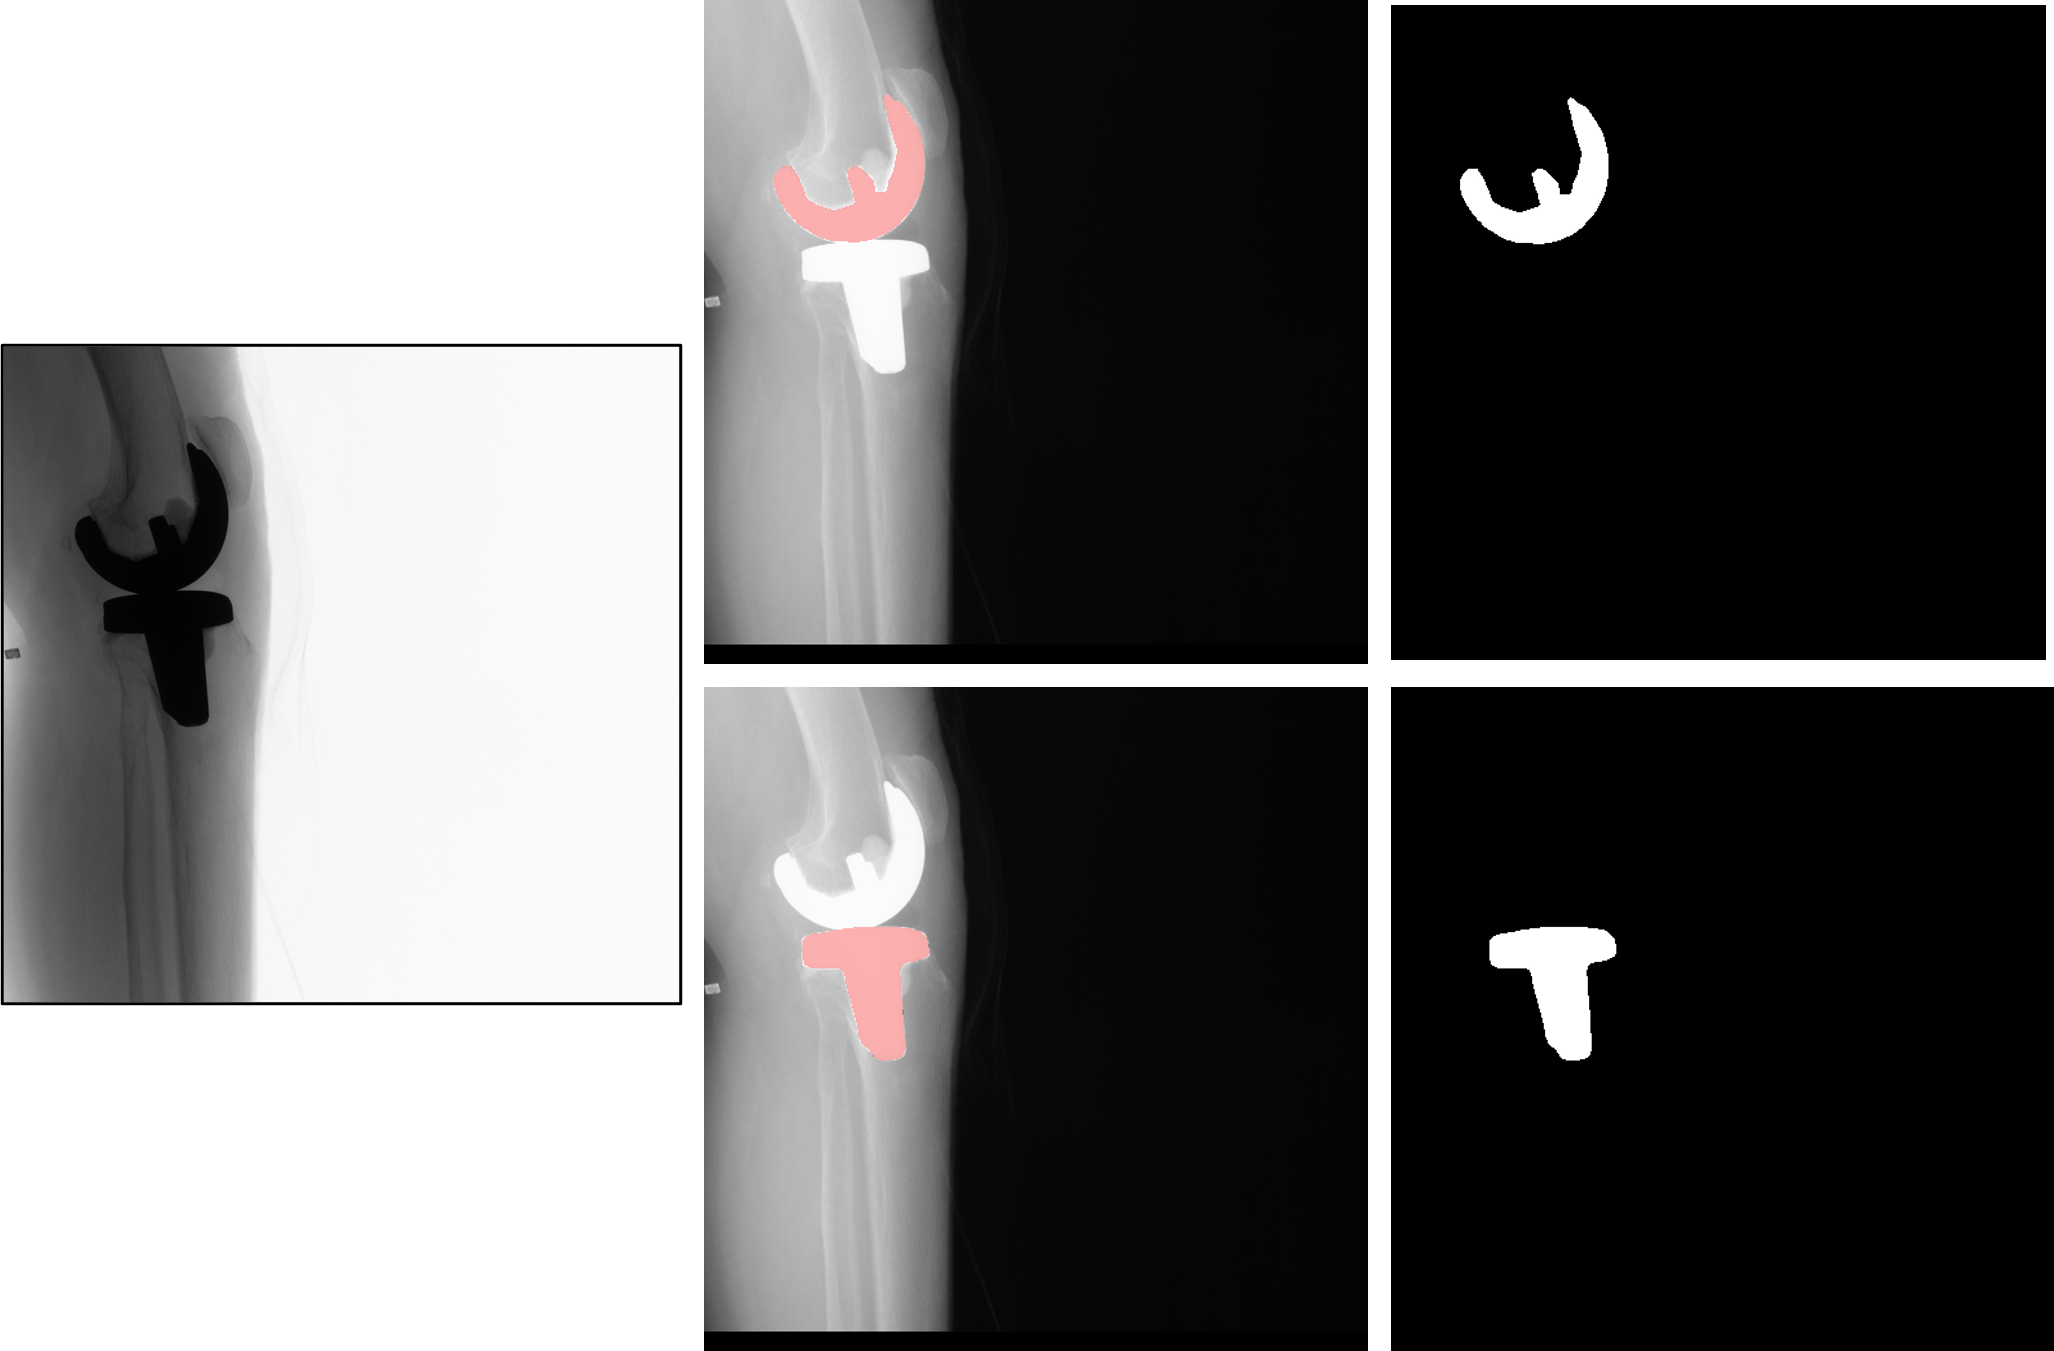
\includegraphics[width=\columnwidth]{/home/ajensen123@ad.ufl.edu/repo/lit-review/figures/raster/jtml-segmentation.png}
\end{center}
\end{column}
\end{columns}
\end{frame}
\begin{frame}[label={sec:org8f17f43}]{Neural Network Data}
\begin{columns}
\begin{column}{0.5\columnwidth}
\begin{itemize}
\item \textasciitilde{}8000 images
\begin{itemize}
\item 7 TKA kinematics studies
\begin{itemize}
\item 71 subjects
\item 7 implant manufacturers
\item 36 distinct implants
\item Squat, lunge, kneel, stair ascent
\end{itemize}
\end{itemize}
\end{itemize}
\end{column}
\begin{column}{0.6\columnwidth}
\begin{center}
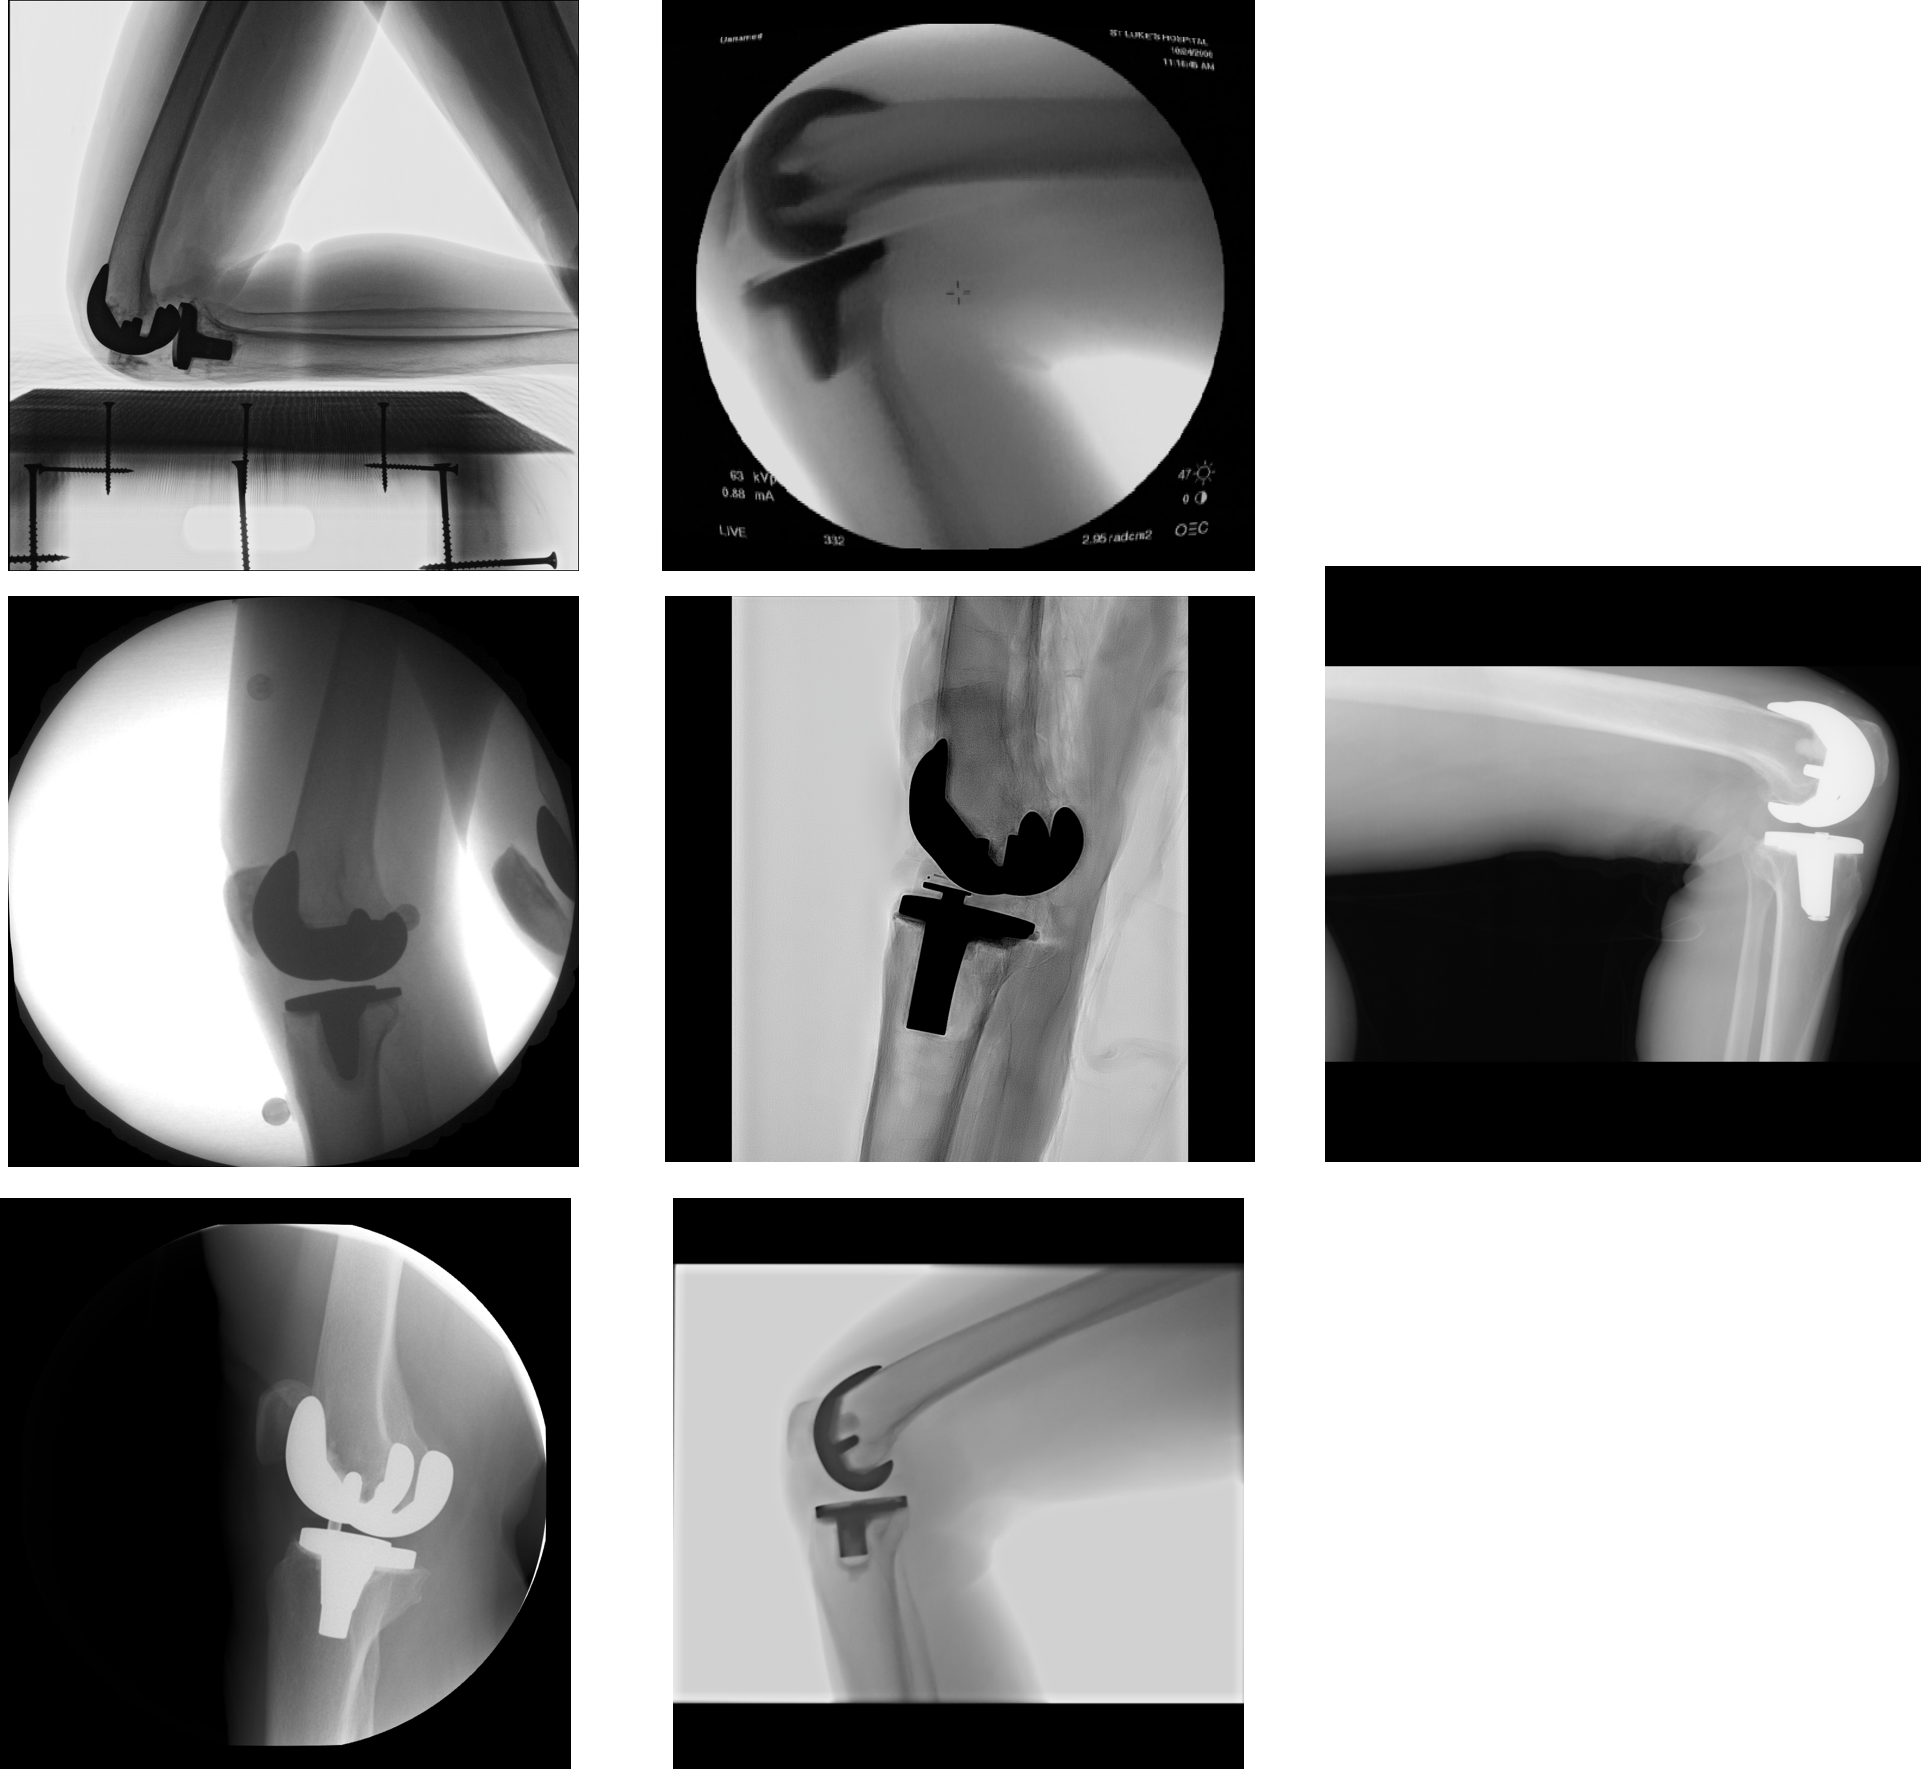
\includegraphics[height=3in]{/home/ajensen123@ad.ufl.edu/repo/lit-review/figures/raster/jtml-data.png}
\end{center}
\end{column}
\end{columns}
\end{frame}
\begin{frame}[label={sec:org353327d}]{Neural Network Robustness}
\begin{itemize}
\item Additional augmentations introduced during training \autocite{buslaevAlbumentationsFastFlexible2020}.
\end{itemize}
\begin{center}
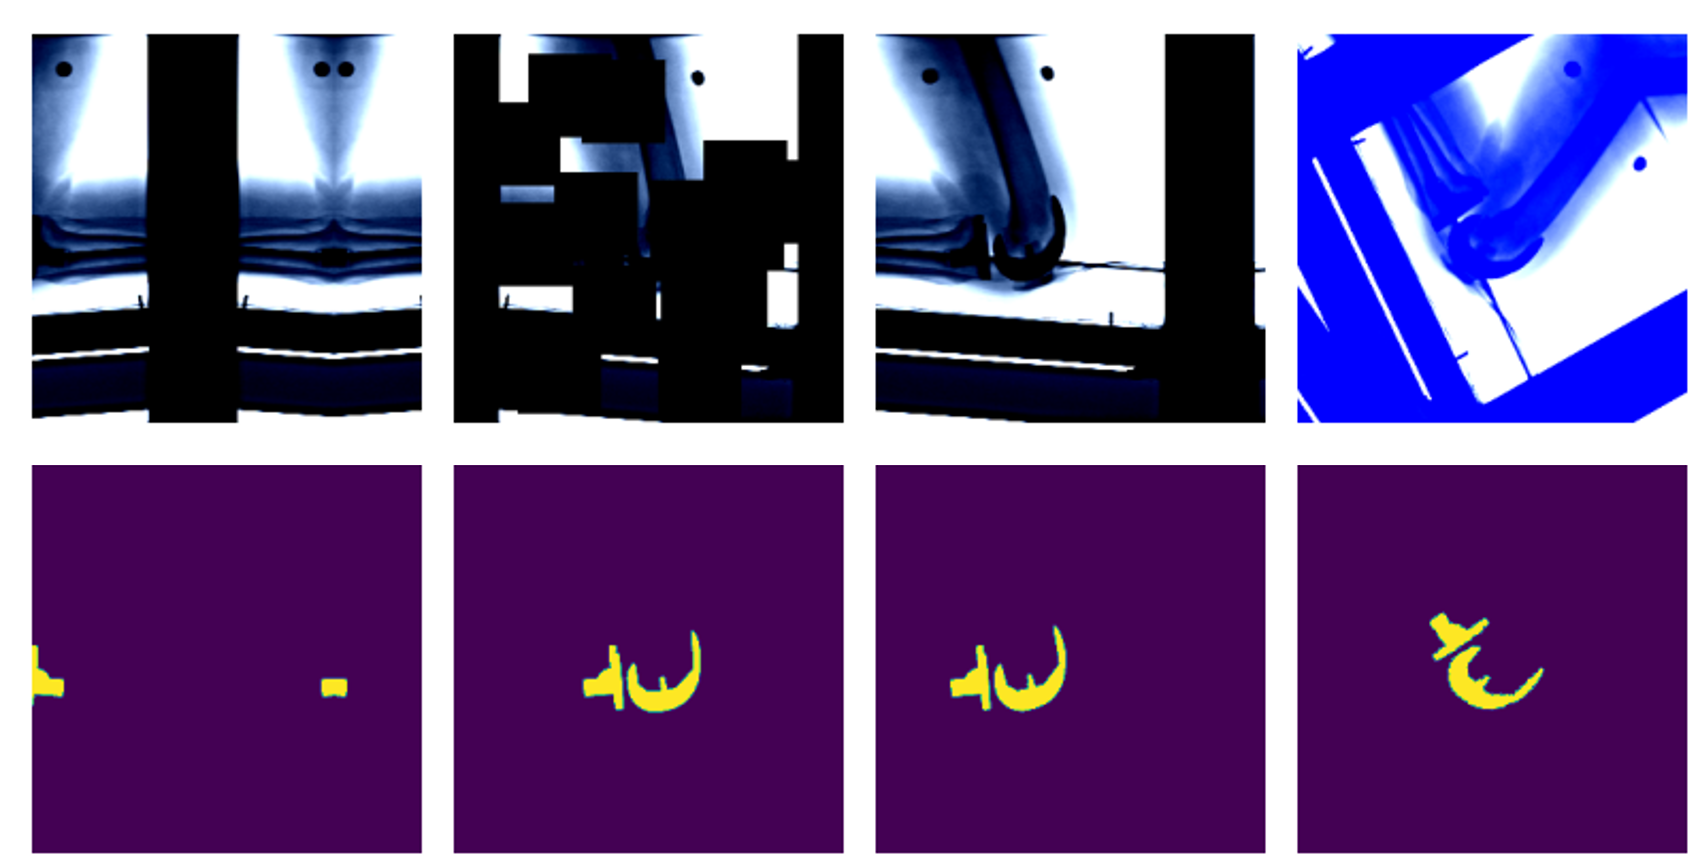
\includegraphics[width=.9\linewidth]{/home/ajensen123@ad.ufl.edu/repo/lit-review/figures/raster/augmentations.png}
\end{center}
\end{frame}
\begin{frame}[label={sec:org2aa0ba4}]{Normalized Fourier Descriptor Shape Libraries}
\begin{columns}
\begin{column}{0.37\columnwidth}
\begin{itemize}
\item Pose initialization using segmentation output.
\item \(\pm 30^{\circ}\) library span at \(3^{\circ}\) increments.
\end{itemize}
\end{column}
\begin{column}{0.7\columnwidth}
\begin{center}
\includegraphics[width=2in]{/home/ajensen123@ad.ufl.edu/repo/lit-review/figures/raster/banks-nfd-library.png}
\end{center}
\begin{center}
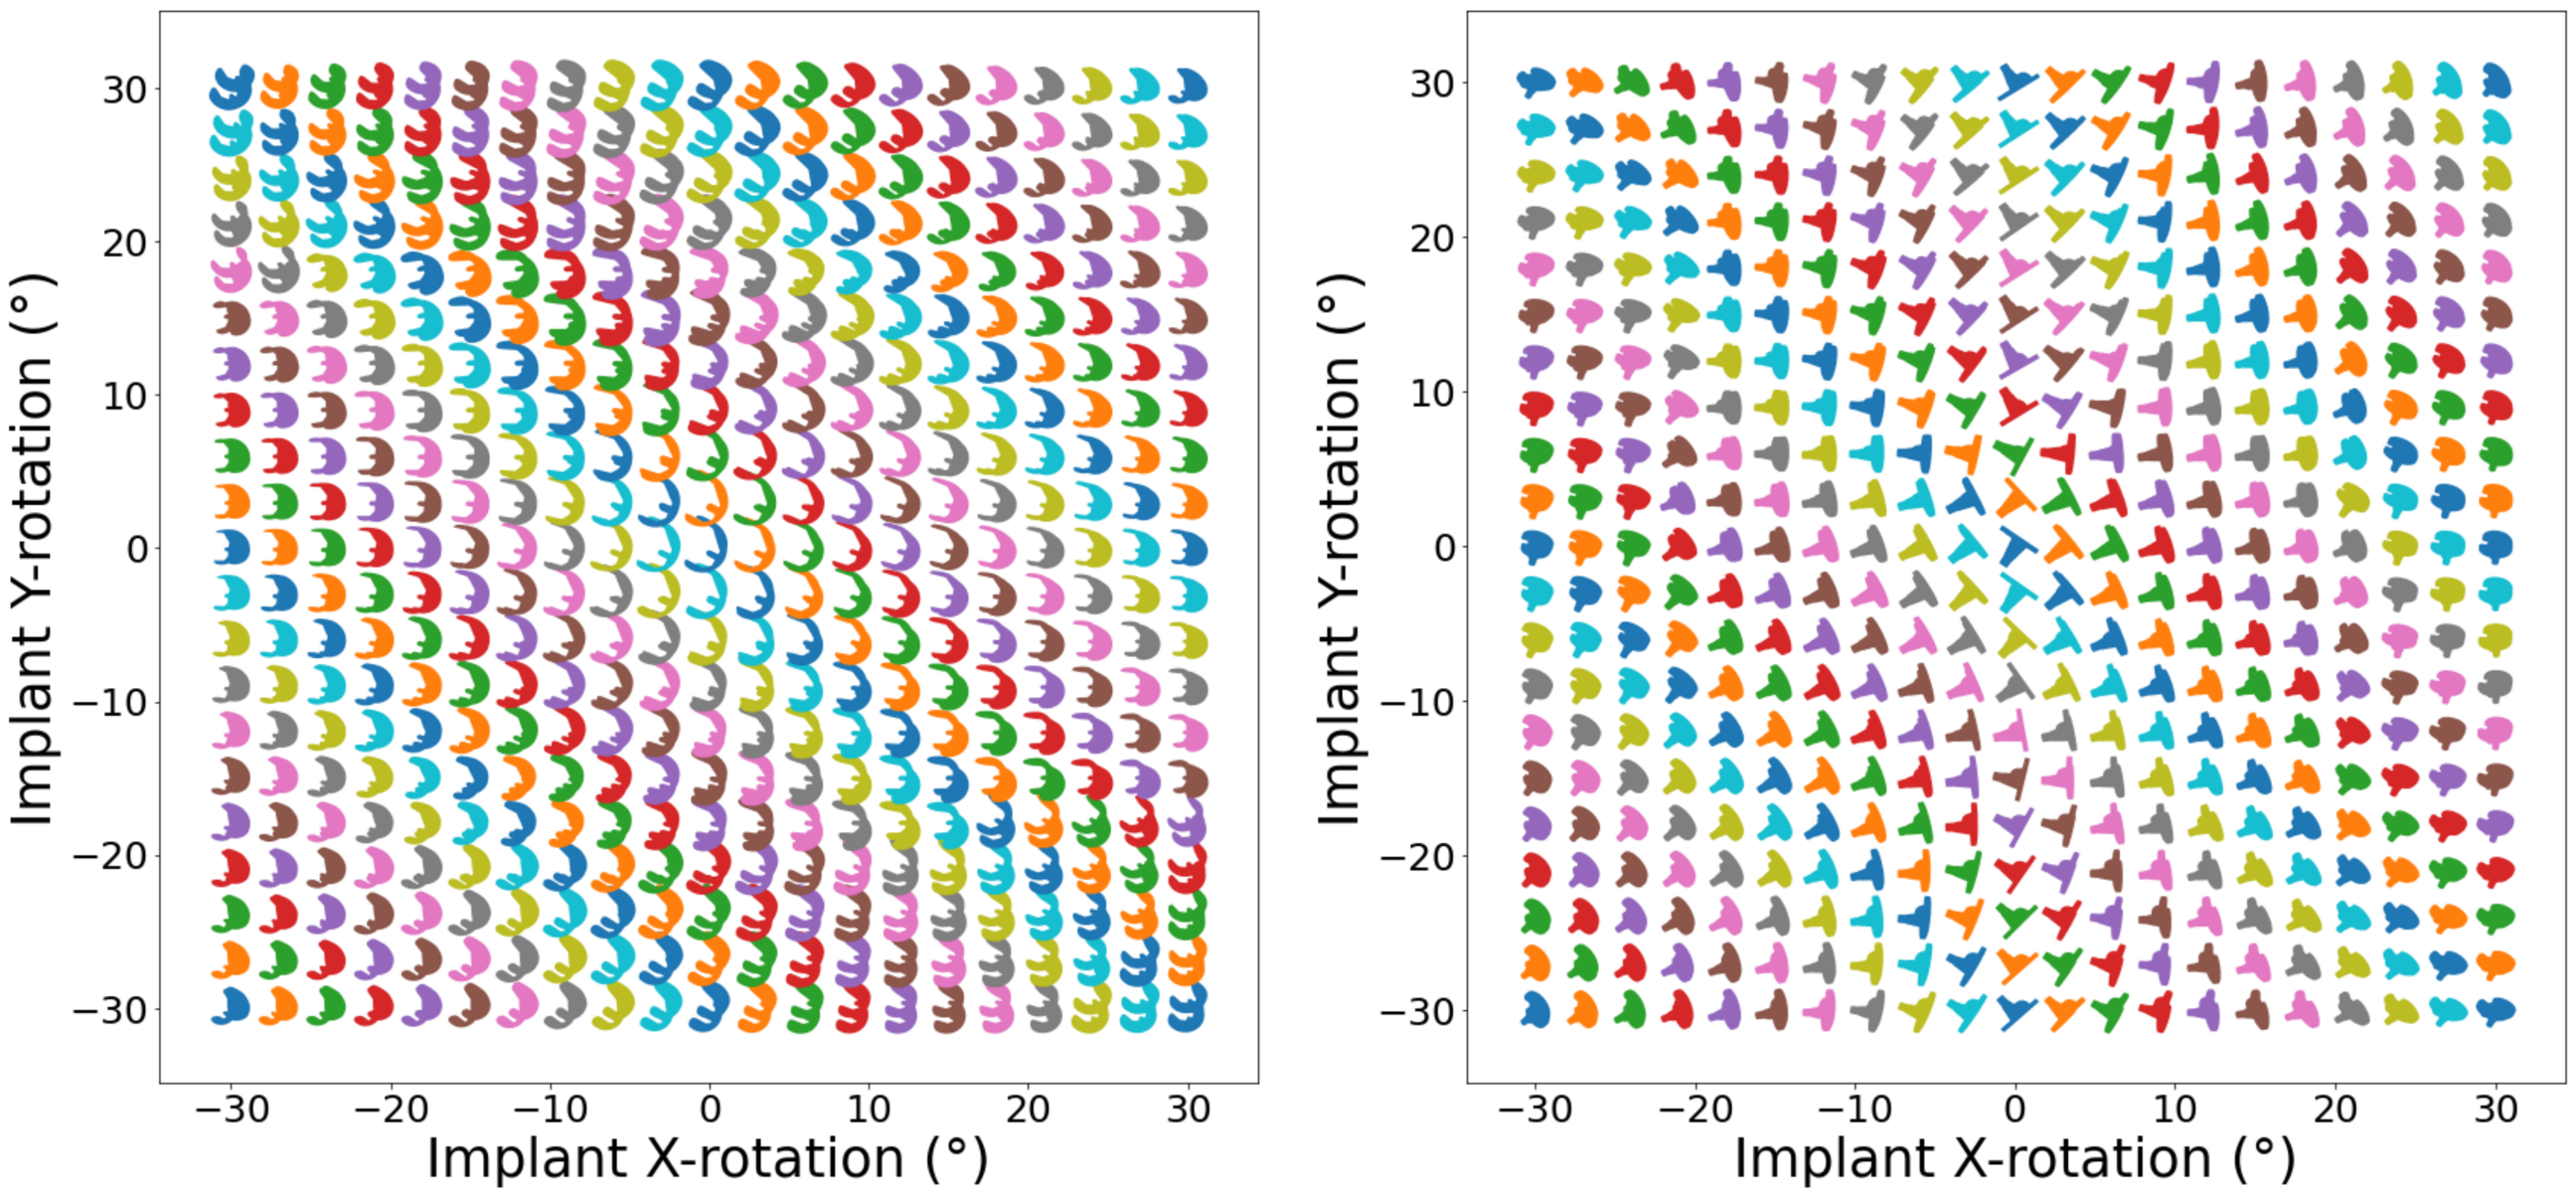
\includegraphics[width=3.25in]{/home/ajensen123@ad.ufl.edu/repo/lit-review/figures/raster/jtml-nfd.png}
\end{center}
\end{column}
\end{columns}
\end{frame}
\begin{frame}[label={sec:org9d37a05}]{Pose Refinement Using Global Optimization}
\begin{columns}
\begin{column}{0.5\columnwidth}
\begin{itemize}
\item Two main features
\begin{itemize}
\item Objective function
\item Optimization routine
\end{itemize}
\end{itemize}
\end{column}
\begin{column}{0.5\columnwidth}
\begin{equation*}
    \argmin_{x}\{f(x) : x \in \Omega\}
\end{equation*}
\end{column}
\end{columns}
\end{frame}
\begin{frame}[label={sec:org65db075}]{Contour-based Objective Function}
\begin{columns}
\begin{column}{0.5\columnwidth}
\begin{itemize}
\item With accurate projection, contours provide a strong heuristic for orientation.
\item Overlapping pixels between CNN segmentation and projected implant.
\begin{itemize}
\item \(L_1\) norm has quick parallel computation.
\end{itemize}
\end{itemize}

\begin{equation*}
  J = \sum_{i \in H}\sum_{j \in W}|I_{ij} - P_{ij}| = L_{1}(I,P)
\end{equation*}

\begin{itemize}
\item Sensitive to minor perturbations
\end{itemize}
\end{column}
\begin{column}{0.6\columnwidth}
\begin{center}
\includegraphics[width=.9\linewidth]{/home/ajensen123@ad.ufl.edu/repo/lit-review/figures/raster/registered-tka.png}
\end{center}
\end{column}
\end{columns}
\end{frame}
\begin{frame}[label={sec:orgf01f1b2}]{Improving Robustness}
\begin{columns}
\begin{column}{0.5\columnwidth}
\begin{itemize}
\item Dilation decreases sensitivity to perturbations.
\item Multi-stage optimization can reduce dilation back to original edges.
\end{itemize}
\end{column}
\begin{column}{0.6\columnwidth}
\begin{center}
\includegraphics[width=\textwidth]{/home/ajensen123@ad.ufl.edu/repo/lit-review/figures/raster/flood-dilated-contour.png}
\end{center}
\end{column}
\end{columns}
\end{frame}
\begin{frame}[label={sec:org4b2ff90}]{Optimization Routine}
\begin{itemize}
\item No analytic form of the objective function exists, it \alert{\alert{must}} be sampled at points of interest.
\begin{itemize}
\item Black Box Optimization \autocites{audetDerivativeFreeBlackboxOptimization2017}[][]{bajajBlackBoxOptimizationMethods2021}
\end{itemize}
\end{itemize}
\end{frame}
\begin{frame}[label={sec:org630b88c}]{Lipschitzian Optimization}
\begin{columns}
\begin{column}{0.5\columnwidth}
\begin{itemize}
\item Robust, global, black-box optimization routine if Lipschitz constant (\(K\)) is known \autocite{shubertSequentialMethodSeeking1972}.
\item Lipschitz constant bounds the rate of change of a function.
\item What if you don't know the Lipschitz constant?
\end{itemize}
\end{column}
\begin{column}{0.6\columnwidth}
\begin{center}
\includegraphics[width=2in]{/home/ajensen123@ad.ufl.edu/repo/lit-review/figures/raster/shubert-step1.png}
\end{center}
\begin{center}
\includegraphics[width=2in]{/home/ajensen123@ad.ufl.edu/repo/lit-review/figures/raster/shubert-step2.png}
\end{center}
\begin{center}
\includegraphics[width=2in]{/home/ajensen123@ad.ufl.edu/repo/lit-review/figures/raster/shubert-step3.png}
\end{center}
\end{column}
\end{columns}
\end{frame}
\begin{frame}[label={sec:orgedeb46c}]{Lipschitzian Optimization without the Lipschitz Constant}
\begin{center}
\includegraphics[width=2.5in]{/home/ajensen123@ad.ufl.edu/repo/lit-review/figures/raster/jones-direct-title.png}
\end{center}
\begin{itemize}
\item Sample end-points instead of intersecting lines.
\item Potentially optimal regions based on value at center and total size.
\begin{itemize}
\item Trisect potentially optimal regions and re-sample centers
\end{itemize}
\end{itemize}
\begin{center}
\includegraphics[width=2.5in]{/home/ajensen123@ad.ufl.edu/repo/lit-review/figures/raster/direct-1D.png}
\end{center}
\end{frame}
\begin{frame}[label={sec:org667bb30}]{Trisecting Region}
\begin{columns}
\begin{column}{0.4\columnwidth}
\begin{equation*}
  \begin{bmatrix}
    f(x=c_{1}) & d(c_{1})\\
    f(x=c_{2}) & d(c_{2})\\
    \vdots & \vdots \\
    f(x=c_{N}) & d(c_{N})
  \end{bmatrix}
\end{equation*}
Where

\begin{align*}
  f(x=c_{i}) &\equiv \text{Sampled function value} \\
  d(c_{i}) & \equiv \text{ Sub-domain size } \\
  & \text{ for } i \in [1,N]
\end{align*}
\end{column}
\begin{column}{0.6\columnwidth}
\begin{center}
\includegraphics[width=\textwidth]{/home/ajensen123@ad.ufl.edu/repo/lit-review/figures/raster/direct-1D-stage1.png}
\end{center}
\end{column}
\end{columns}
\end{frame}
\begin{frame}[label={sec:orgb4188b8}]{Another Iteration}
\begin{columns}
\begin{column}{0.4\columnwidth}
\begin{equation*}
  \begin{bmatrix}
    f(x=c_{1}) & d(c_{1})\\
    f(x=c_{2}) & d(c_{2})\\
    \vdots & \vdots \\
    f(x=c_{N}) & d(c_{N})
  \end{bmatrix}
\end{equation*}
Where

\begin{align*}
  f(x=c_{i}) &\equiv \text{Sampled function value} \\
  d(c_{i}) & \equiv \text{ Sub-domain size } \\
  & \text{ for } i \in [1,N]
\end{align*}
\end{column}
\begin{column}{0.6\columnwidth}
\begin{center}
\includegraphics[width=\textwidth]{/home/ajensen123@ad.ufl.edu/repo/lit-review/figures/raster/direct-1D-stage2.png}
\end{center}
\end{column}
\end{columns}
\end{frame}
\begin{frame}[label={sec:org3801fb4}]{Determining Potentially Optimal Regions}
\begin{itemize}
\item Convex hull \autocites{grahamEfficientAlgorithDetermining1972}[][]{jarvisIdentificationConvexHull1973}[][]{chanOptimalOutputsensitiveConvex1996}[][]{barberQuickhullAlgorithmConvex1996} of region size vs. center value
\end{itemize}

\begin{center}
\includegraphics[width=0.6\textwidth]{/home/ajensen123@ad.ufl.edu/repo/lit-review/figures/raster/direct-convex-hull.png}
\end{center}
\end{frame}
\begin{frame}[label={sec:orgca5803b}]{DiRECT for Joint Track Machine Learning}
\begin{itemize}
\item Search region is along all 6 degrees of freedom.
\begin{itemize}
\item Normalize to \([0,1]\).
\end{itemize}
\item Three stages, each with decreasing levels of dilation.
\begin{itemize}
\item Iteration budget for each stage.
\end{itemize}
\end{itemize}
\begin{center}
\begin{tabular}{lllr}
Stage & Budget [Iterations] & Search Range [mm,deg] & Dilation (pixels)\\
\hline
``Tree'' & \textasciitilde{}20,000 & \(\pm 45\) & 5\\
``Branch'' & \textasciitilde{}20,000 & \(\pm 25\) & 3\\
``Leaf'' & \textasciitilde{}10,000 & \(\pm 100\) \((z_{trans})\) / \(\pm 3\) \((else)\) & 1\\
\end{tabular}
\end{center}
\end{frame}
\begin{frame}[label={sec:org31f1c30}]{Testing Performance}
Now that we have our refined poses, how well does out system perform?
\begin{center}
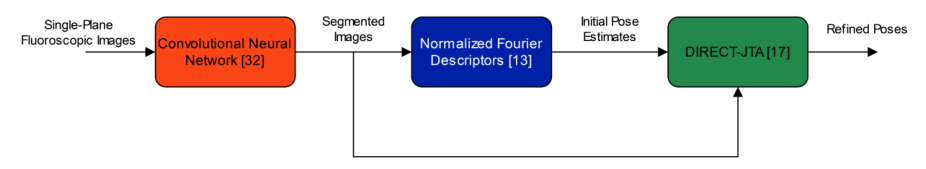
\includegraphics[width=\textwidth]{/home/ajensen123@ad.ufl.edu/repo/lit-review/figures/raster/jtml-pipeline.png}
\end{center}
\end{frame}
\begin{frame}[label={sec:orgb012e8e}]{Validation}
\begin{itemize}
\item Independent research group using Model-Based RSA.
\item Determine the level of concordance between the two measurement systems
\begin{itemize}
\item Bland-Altmann Plots
\end{itemize}
\item Achieved clinically acceptable accuracy \autocites{brobergValidationMachineLearning2023}[][]{jensenJointTrackMachine2022}.
\item Highly repeatable
\end{itemize}

\begin{center}
\includegraphics[width=0.7\textwidth]{/home/ajensen123@ad.ufl.edu/repo/lit-review/figures/raster/broberg-bland-altmann.png}
\end{center}
\end{frame}
\begin{frame}[label={sec:org64d1651}]{Awards}
The work presented in this aim won the HAP Paul Award for Best Paper from the International Society for Technology in Arthroplasty's 2022 Annual Meeting.
\begin{center}
\includegraphics[width=0.7\textwidth]{/home/ajensen123@ad.ufl.edu/repo/lit-review/figures/raster/ista-hap-paul-talk.png}
\end{center}
\end{frame}
\subsection{Aim 2 - Overcoming Single-Plane Limitations}
\label{sec:org73a4772}
\begin{frame}[label={sec:orgeb6bc01}]{Goal}
\begin{itemize}
\item The goal of this aim is to validate and test methods that can overcome single-plane limitations for model-image registration.
\begin{itemize}
\item Out-of-plane (OOP) Translation
\item Symmetry Traps
\end{itemize}
\end{itemize}
\end{frame}
\begin{frame}[label={sec:org2b445ce}]{Translation}
\begin{itemize}
\item Depth perception is lost when using a single camera.
\item Utilize a virtual ``spring'' to constrain relative OOP translation between implant components.
\end{itemize}

\begin{equation*}
  J = \alpha L_{1}(I,P) + \beta ML(Fem,Tib)
\end{equation*}

Where
\begin{equation*}
  ML \equiv \text{ Relative mediolateral translation }
\end{equation*}
\end{frame}
\begin{frame}[label={sec:org245a49f}]{Symmetry Traps}
With a symmetric tibial implant, the contour is not always a perfect heuristic for true pose. Human operators typically utilize relative varus-valgus to determine correct pose.

Found ``ambiguous zone'' within \(3^{\circ}\) of pure lateral pose with high propensity for symmetry traps \autocite{jensenJointTrackMachine2022}.

\begin{center}
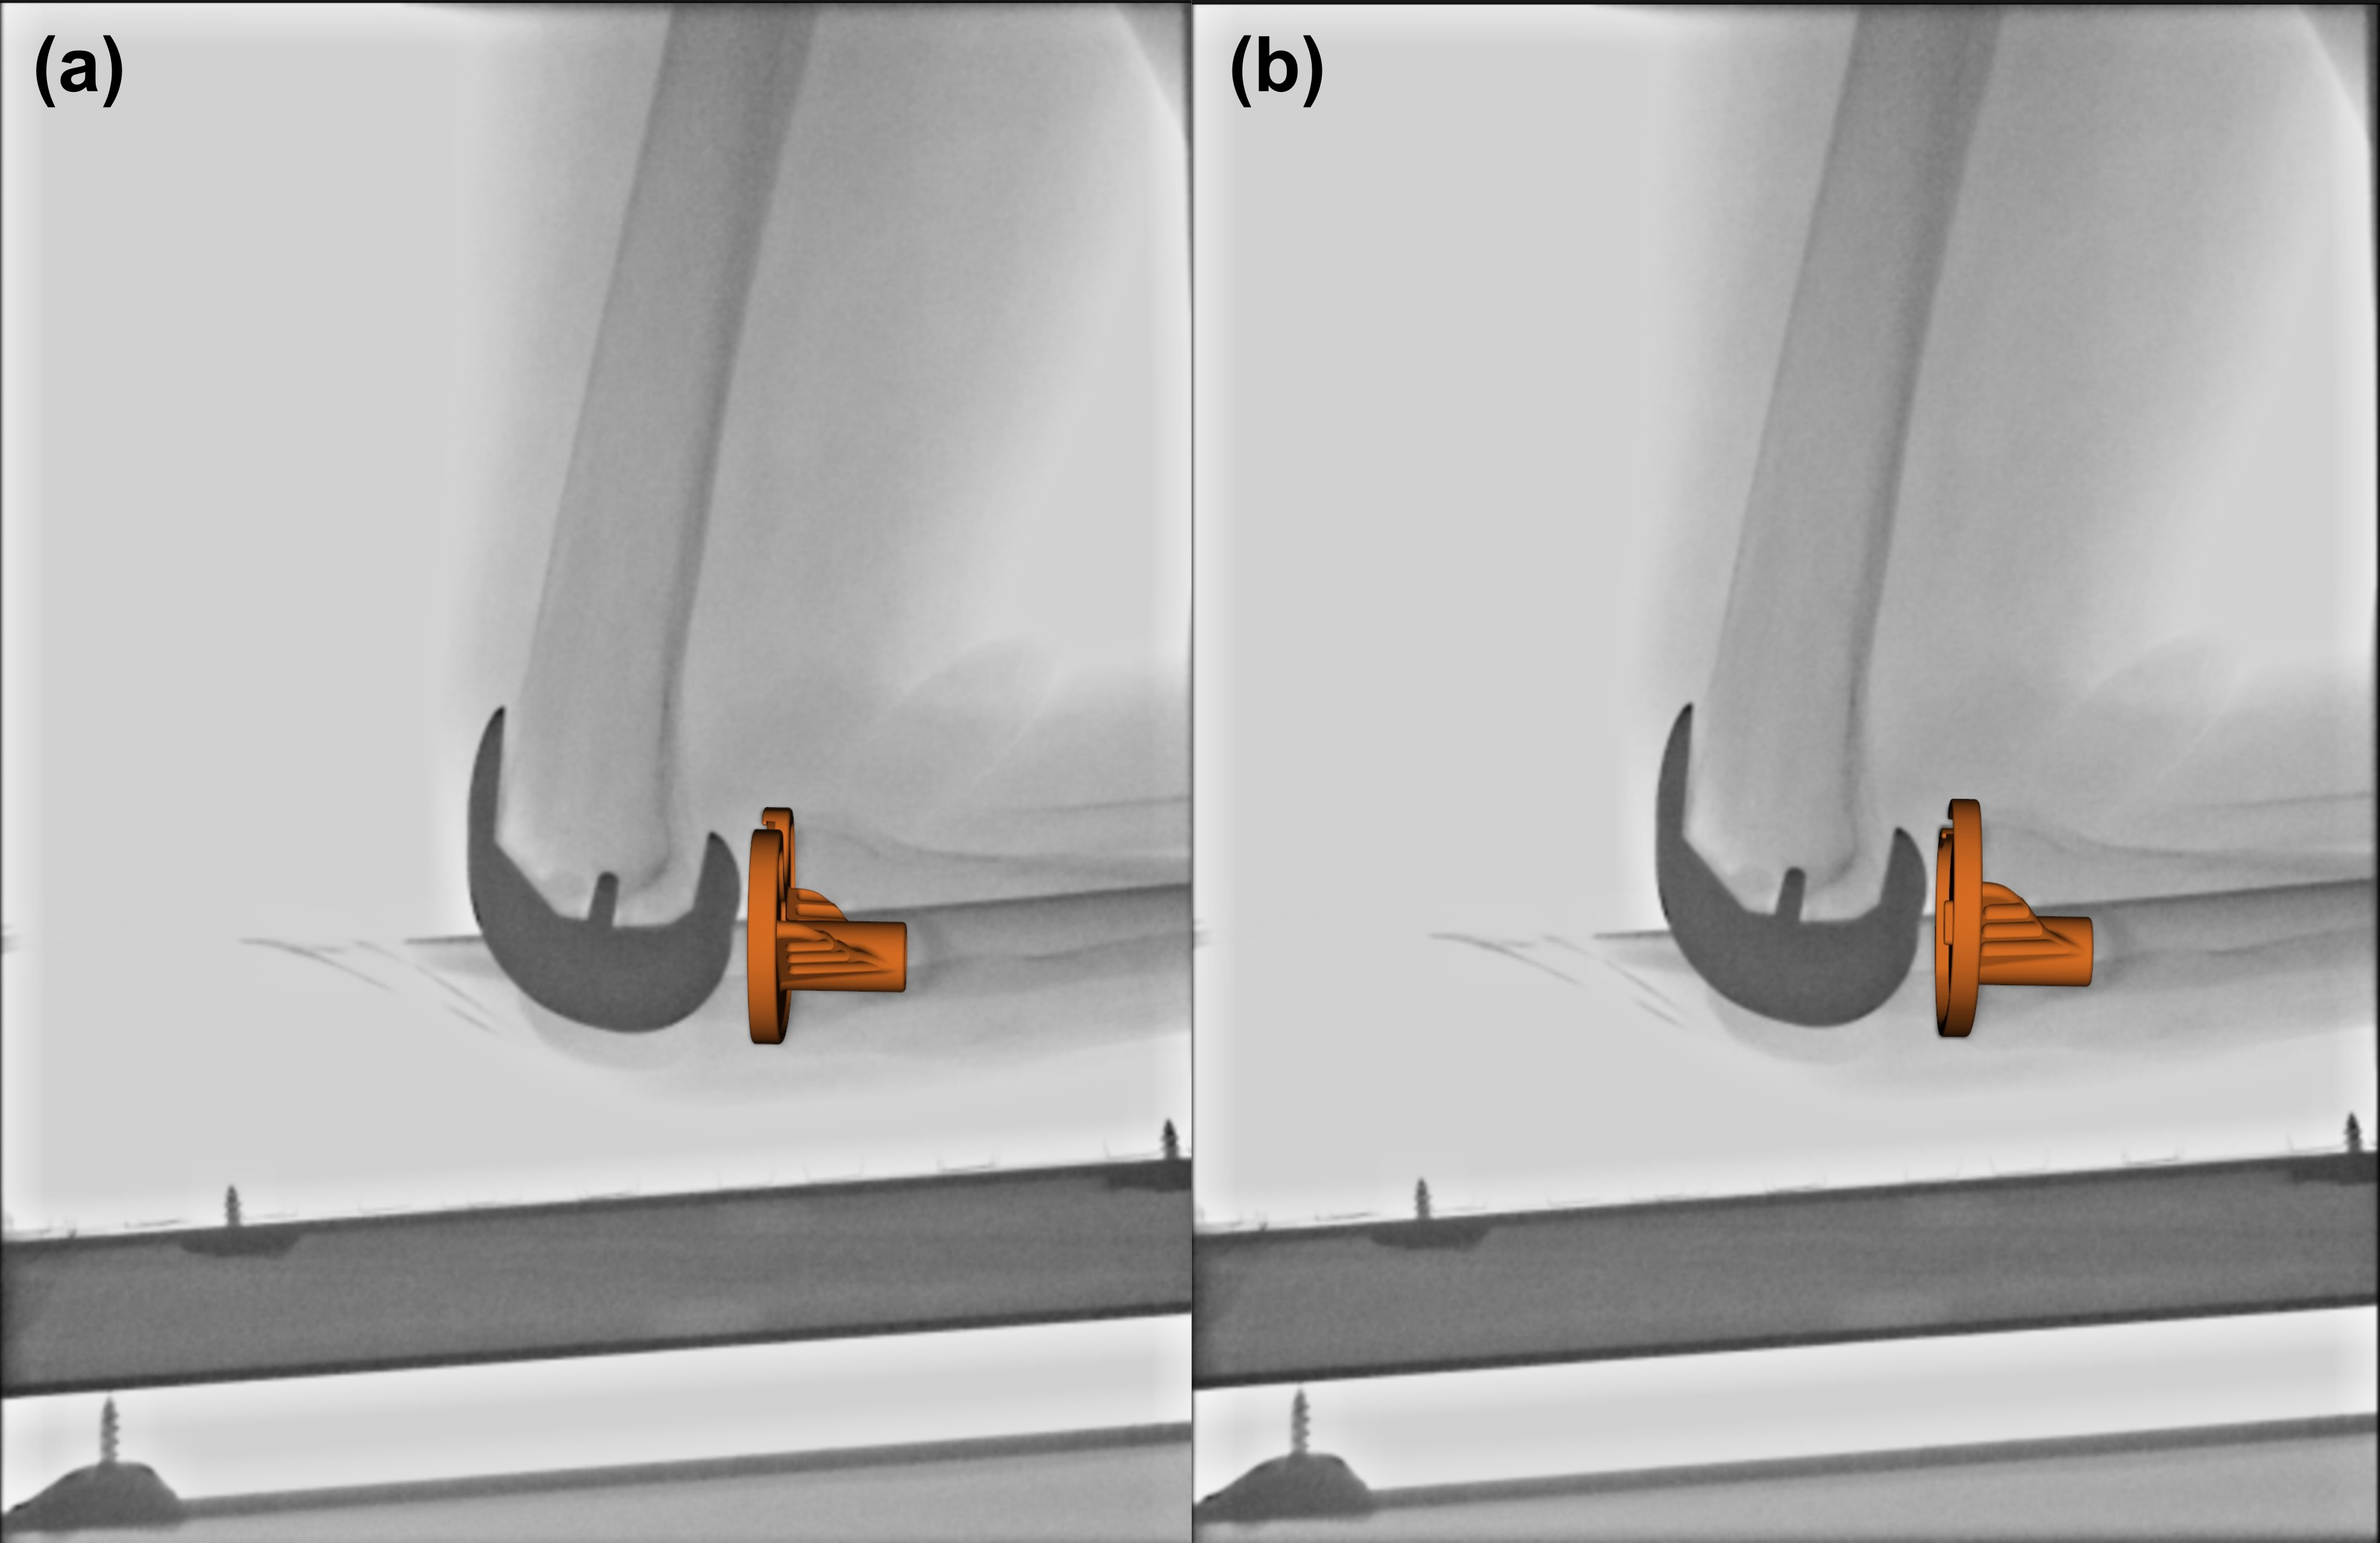
\includegraphics[width=0.7\textwidth]{/home/ajensen123@ad.ufl.edu/repo/lit-review/figs/jtml-paper/fig6-symtrap.png}
\end{center}
\end{frame}
\begin{frame}[label={sec:orga16edcd}]{Solving the Symmetric Pose}
\begin{columns}
\begin{column}{0.5\columnwidth}
Algorithm devised to ``flip'' pose into symmetric counterpart.
\begin{enumerate}
\item Determine viewing ray from camera to implant centroid, denote \(\vec{v}\), normalize.
\item Denote symmetric-plane normal vector \(\vec{s}\), normalize.
\item Measure relative ``off-lateral'' orientation of implant, \(\cos(\theta) = \dfrac{\vec{v} \cdot \vec{s}}{||\vec{v} || ||\vec{s} || }\)
\item Apply body-centered rotation to implant about \(\vec{m} = \vec{s} \times \vec{v}\) by \(\psi = 2\theta\).
\end{enumerate}
\end{column}
\begin{column}{0.6\columnwidth}
\begin{center}
\includegraphics[width=0.6\textwidth]{/home/ajensen123@ad.ufl.edu/figures/raster/symmetry_flipper.png}
\end{center}
\end{column}
\end{columns}
\end{frame}
\begin{frame}[label={sec:org6b63e20}]{Four Approaches}
\begin{itemize}
\item Virtual ligaments
\item Binary selection between two poses
\item Bland-Altmann Calibration Constant
\item Fully Connected Network
\end{itemize}
\end{frame}
\begin{frame}[label={sec:orgbc630a1}]{Virtual Ligaments}
\begin{equation*}
  J = \alpha L_{1}(I,P) + \beta ML(Fem,Tib) + \gamma VV(Fem,Tib)
\end{equation*}

Where

\begin{equation*}
  VV \equiv \text{  Relative Varus-Valgus rotation}
\end{equation*}
\end{frame}
\begin{frame}[label={sec:org236f094}]{Binary Selection}
\begin{enumerate}
\item Determine optimized pose using \(L_1 + ML\)
\item Calculate symmetric pose.
\item Pick pose with lower relative VV
\end{enumerate}

This method can simplify the selection criteria (one fewer hyperparameter).
\end{frame}
\begin{frame}[label={sec:orgfa27138}]{Bland-Altmann Calibration Constant}
\begin{itemize}
\item Utilizing Bland-Altmann plots from gold-standard kinematics, create a ``correction constant'' for relative varus/valgus (ad/abduction) angles.
\item Notice linear trend in BA plots.
\end{itemize}
\begin{center}
\includegraphics[width=0.75\textwidth]{/home/ajensen123@ad.ufl.edu/repo/lit-review/figures/raster/broberg-bland-altmann.png}
\end{center}
\end{frame}
\begin{frame}[label={sec:orgc1bd81a}]{Fully Connected Network}
\begin{columns}
\begin{column}{0.5\columnwidth}
\begin{itemize}
\item Encode symmetric pose calculation into FCN.
\item Feed femoral and tibial \alert{\alert{pose}} into network.
\begin{itemize}
\item ``Keep'' or ``Switch''
\end{itemize}
\item Could incorporate categorical features as well
\begin{itemize}
\item Weightbearing vs non-weightbearing
\item Activity (walking, stair, lunge, etc)
\end{itemize}
\end{itemize}
\end{column}
\begin{column}{0.6\columnwidth}
\begin{center}
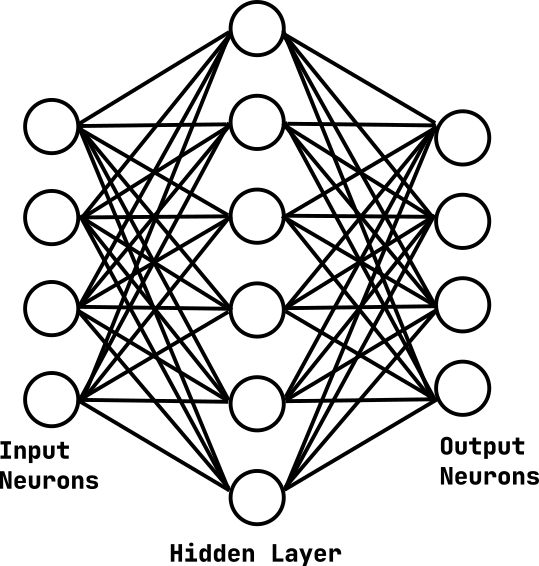
\includegraphics[width=2.2in]{/home/ajensen123@ad.ufl.edu/repo/lit-review/figures/raster/fcn.png}
\end{center}
\end{column}
\end{columns}
\end{frame}
\begin{frame}[label={sec:orgd36fe92}]{Timeline}
\begin{itemize}
\item All kinematics data has already been collected.
\item Completed Methods
\begin{itemize}
\item Virtual Ligaments
\end{itemize}
\item In Progress
\begin{itemize}
\item Binary Selection
\end{itemize}
\item Pending Methods
\begin{itemize}
\item Bland-Altmann Calibration
\item Fully Connected Network
\end{itemize}
\end{itemize}

Journal paper will be ready for submission by June.
\end{frame}
\subsection{Aim 3 - Pilot Human Study}
\label{sec:orgf828fac}
\begin{frame}[label={sec:org7cf5b36}]{Goal}
No kinematics studies have exclusively utilized Joint Track Machine Learning; let's be the first.

What are we measuring?
\begin{itemize}
\item Kinematics
\item Time to full examination report
\begin{itemize}
\item Time/frame
\item Usage hiccups
\item Symmetry traps
\end{itemize}
\end{itemize}
\end{frame}
\begin{frame}[label={sec:org3057ca8}]{Methods}
\begin{itemize}
\item 20-30 patients
\item \textasciitilde{}Dozen activities with fluoroscopic machine
\begin{itemize}
\item Weightbearing and Non-weightbearing
\item Static and Dynamic
\end{itemize}
\end{itemize}

IRB approval \textasciitilde{}4 months out.
\end{frame}
\subsection{Aim 4 - Standardized Kinematics Exam}
\label{sec:org32c8afb}
\begin{frame}[label={sec:org31479a5}]{Goal}
Establish a ``standard kinematics exam'' by determining the most statistically and anatomically relevent fluoroscopic image(s) to capture during a clinical visit.
\end{frame}
\begin{frame}[label={sec:orgcceefd2}]{Motivation}
\begin{itemize}
\item We have standardized pain/outcome scores
\begin{itemize}
\item KOOS, KSS, FJS, etc..
\end{itemize}
\item No standardized kinematics examination
\begin{itemize}
\item Per-study differences
\item No reason to standardize
\end{itemize}
\end{itemize}

Autonomous kinematics measurements allow researchers to spend more time asking and answering questions rather than fiddling with annoying software.
\end{frame}
\begin{frame}[label={sec:org159ad09}]{Method}
\begin{itemize}
\item Use images and kinematics from Aim 3.
\item Utilize statistical methods to determine covariance and causal/corollary relationships.
\begin{itemize}
\item Clustering
\item Transformers \autocites{carionEndtoEndObjectDetection2020}[][]{vaswaniAttentionAllYou2017}[][]{guoAttentionMechanismsComputer2021}[][]{dosovitskiyImageWorth16x162021} (``translating'' movements into outcomes and other movements)
\end{itemize}
\end{itemize}
\end{frame}
\subsection{Aim 5 - Joint Track Auto Toolkit}
\label{sec:org0c7cdb8}
\begin{frame}[label={sec:orge63743a}]{Joint Track Auto Toolkit (JTAT)}
Create a freely available Python library that allows other researchers to utilize JTML's model-image registration framework. Extra emphasis will be placed on extensibility to allow other researchers to compose their own registration pipelines.
\end{frame}
\begin{frame}[label={sec:org7964be5},fragile, allowframebreaks, label=]{Presentations}
\begin{refsection}
  
\nocite{%
banksRegioneCaecorumRex2019,  daiComparativeAnalysisFixation2021, daiImpactFixationComponents2021, floodPracticalClinicalExamination2019, griffithAutomatedSegmentationGrading2022, jensenAutonomousMeasurement3D2022, jensenAutonomousMethodExtracting2021, jensenAutonomousMethodExtracting2021a, jensenComparisonClinicalComputational2020, jensenDeepLearningImage2023,  jensenRoutineClinicalExamination2020,jensenImpactSagittalResection2020}

  \printbibliography[title=Presentations]
\end{refsection}
\end{frame}
\begin{frame}[label={sec:org4284335},fragile, allowframebreaks, label=]{Publications}
\begin{refsection}
  
\nocite{%
brobergValidationMachineLearning2023, burtonAutomaticTrackingHealthy2021, jensenJointTrackMachine2022,
}

  \printbibliography[title=Publications]
\end{refsection}
\end{frame}
\begin{frame}[label={sec:org8556f7e}]{Timeline}
\begin{center}
\begin{tabular}{ll}
Date(s) & Event\\
\hline
2015-2019 & Mech. Eng. B.S, Magna Cum Laude, UF\\
April 2019 - April 2020 & Internship at Exactech\\
April 2020 & Started in Miller Lab\\
August 2020 & Officially Started PhD at UF\\
November 2021 & Best Presentation Award at ISTA: Emerging Technologies\\
April 2022 & Submitted JTML for HAP Paul Award\\
September 2022 & HAP Paul Award at ISTA 2022\\
\hline
June 2023 & Single-plane limitations paper submitted\\
July 2023 & Est. IRB Approval\\
August 2023 & v1.0 JTAT\\
December 2023 \textasciitilde{} May 2024 & Patient Data Fully Collected (Aims 3/4)\\
August 2024 & Papers for Aims 3/4 Submitted\\
December 2024 - April 2025 & Est. Graduation\\
\end{tabular}
\end{center}
\end{frame}
\begin{frame}[label={sec:orga3621d4},standout]{Thank you!}
Thanks for listening!!
\end{frame}
\section{References}
\label{sec:org63d3dff}
\begin{frame}[label={sec:org59f4e8a},fragile, allowframebreaks, label=]{References}
\AtNextBibliography{\tiny}
\printbibliography
\end{frame}
\end{document}
